\documentclass[tikz,border=2pt]{standalone}
\usepackage{amsmath,amssymb}
\usepackage{pgfplots}
\pgfplotsset{compat=1.18}

\begin{document}
% Bin(100, 0.5) drawn as unit-width bars with the N(50, 25) density. The bars for 45..55 cover
% the interval [44.5, 55.5], so the normal area is taken between the half-unit points.
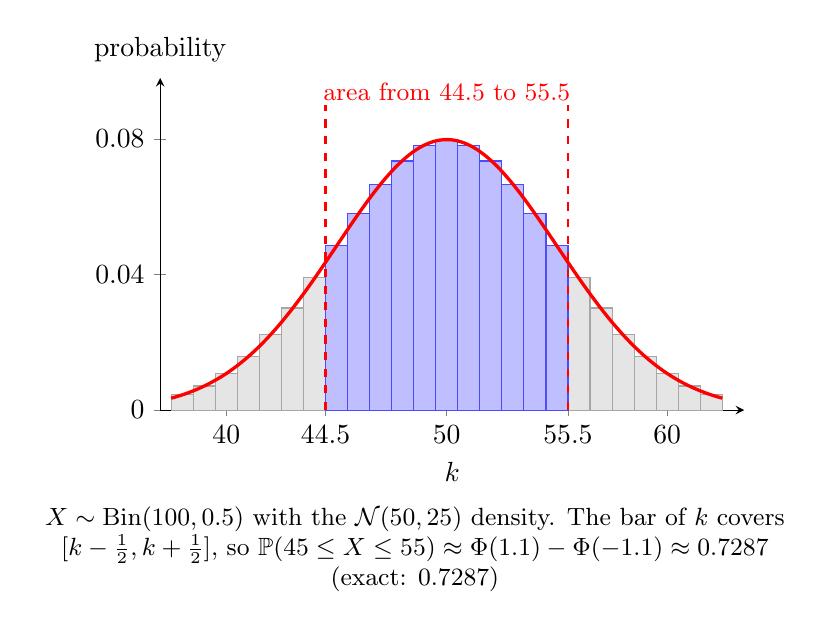
\begin{tikzpicture}
	\begin{axis}[
		axis lines=left, xmin=37, xmax=63.5, ymin=0, ymax=0.098,
		xtick={40,44.5,50,55.5,60}, xticklabels={$40$,$44.5$,$50$,$55.5$,$60$}, ytick={0,0.04,0.08},
		yticklabel style={/pgf/number format/fixed, /pgf/number format/precision=2}, scaled y ticks=false,
		xlabel={$k$}, ylabel={probability}, ylabel style={rotate=-90, anchor=south, at={(axis description cs:0,1.02)}},
		width=9cm, height=5.8cm, clip=false
		]
		\addplot[ybar, bar width=1, fill=gray!20, draw=gray!70] coordinates {(38,0.0045) (39,0.0071) (40,0.0108) (41,0.0159) (42,0.0223) (43,0.0301) (44,0.0390) (56,0.0390) (57,0.0301) (58,0.0223) (59,0.0159) (60,0.0108) (61,0.0071) (62,0.0045)};
		\addplot[ybar, bar width=1, fill=blue!25, draw=blue!70] coordinates {(45,0.0485) (46,0.0580) (47,0.0666) (48,0.0735) (49,0.0780) (50,0.0796) (51,0.0780) (52,0.0735) (53,0.0666) (54,0.0580) (55,0.0485)};
		\addplot[red, very thick, domain=37.5:62.5, samples=120, smooth] {exp(-(x-50)^2/50)/(5*sqrt(2*pi))};
		\draw[red, dashed, thick] (axis cs:44.5,0) -- (axis cs:44.5,0.09);
		\draw[red, dashed, thick] (axis cs:55.5,0) -- (axis cs:55.5,0.09);
		\node[red, anchor=south, font=\small] at (axis cs:50,0.0885) {area from $44.5$ to $55.5$};
	\end{axis}
	\node[anchor=north, font=\small, align=flush center, text width=9.6cm] at ([yshift=-2pt]current axis.outer south) {$X\sim\operatorname{Bin}(100,0.5)$ with the $\mathcal{N}(50,25)$ density. The bar of $k$ covers $[k-\tfrac12,k+\tfrac12]$, so $\mathbb{P}(45\le X\le55)\approx\Phi(1.1)-\Phi(-1.1)\approx0.7287$ (exact: $0.7287$)};
\end{tikzpicture}
\end{document}
